\input{style/settings}
\input{style/short_commands}
\pagestyle{fancy}
\fancyhf{}
\fancyhead[R]{página\;\thepage/\pageref{LastPage}}
\fancyhead[L]{Osvaldo Uriel Calderón Dorantes}
\fancyfoot[L]{Seguridad Radiológica}
\fancyfoot[R]{Facultad de Ciencias, UNAM 
\includegraphics[scale=0.13]{style/Sheikah.pdf}}
\fancypagestyle{plain}{
  \fancyfoot[C]{}
}
\makeatletter
\def\@seccntformat#1{%
  \expandafter\ifx\csname c@#1\endcsname\c@section\else
  \csname the#1\endcsname\quad
  \fi}
\makeatother
%%%%%%%%%%%%%%%%%%%%%%%%%%%%%%%%%%%%%%%%%%%%%%%%%%%%%%%
%%%%%%%%%%%%%%%%%%%%%%%%%%%%%%%%%%%%%%%%%%%%%%%%%%%%%%%%%%%
\begin{document}
\begin{flushleft}
Osvaldo Uriel Calderón Dorantes, \hfill Seguridad Radiológica\\
316005171 \hfill osvaldo13576@ciencias.unam  \\
Facultad de Ciencias\\
\underline{Universidad Nacional Autónoma de México}
\end{flushleft}

\begin{flushright}\vspace{-5mm}

\includegraphics[height=1.5cm]{style/logo.pdf}
\end{flushright}
 
\begin{center}\vspace{-1cm}
\textbf{ \large \customfont{Práctica 3\\
Detectores de radiación y levantamiento de niveles}}\\
\today
\end{center}
%\medskip\hrule\medskip
%%%%%%%%%%%%%%%%%%%%%%%%%%%%%%%%%%%%%%%%%%%%%%%%
%{\small \textbf{Nota: A las unidades las pondré dentro de corchetes \ec{[\tx{unidad}]} para no confundir entre variables y realizar el análisis dimensional fácilmente.}}
\medskip\hrule

\newlength{\strutheight}
\settoheight{\strutheight}{\strut}


\begin{abstract}
  Mediante detectores de radiación de Pancake Geiger-Muller se realizaron medidas de exposición \ec{X} de una fuente de \ec{^{99m}}Tc dentro de una jeringa la cual estaba encapsulada en un contenedor de transporte de tecnecio, de tal manera que se trabajó con una fuente cerrada ya que no hubo contacto directo con el material y se encontraba dentro de su contenedor.
\end{abstract}
\hrule
\begin{multicols}{2}


  \section{Introducción}
  \subsection*{Exposición \texorpdfstring{\ec{X}}{TEXT}}

  La exposición se define como la suma de cargas de todos los iones producidos en aire por rayos-X o radiación gamma cuando todos los electrones liberados por fotones se detienen completamente en un elemento infinitesimal de volumen de aire  dividido entre la masa de dicho volumen, es decir, expresa la cantidad de carga de electrones (\ec{Q}) por unidad de masa de aire (\ec{m}), se muestra en la ecuación \ref{eq:01}. Su unidad es el Roentgen el cual en el SI equivale como se muestra en la ecuación \ref{eq:02} \citep{conceptos1}.
  \eq{eq:01}{X=\dfrac{dQ}{dm}}
  \eq{eq:02}{1\un{R}=2.58\times10^{-4}\un{C\ec{\cdot}kg\ec{^{-1}}}}
  \subsubsection*{Rapidez de Exposición \texorpdfstring{\ec{\dot{X}}}{TEXT}}

  La rapidez de exposición es la cantidad de exposición por unidad de tiempo en un punto \ec{P}, dada en la ecuación \ref{eq:03}. Su unidad en detectores usualmente son los \ec{\un{mR\ec{\cdot}h\ec{^{-1}}}} \citep{attix}.
  \eq{eq:03}{\dot{X}=\dfrac{dX}{dt}}


  \subsubsection*{Ley del inverso cuadrado}

  Dada una fuente puntual, la velocidad de exposición se describe como se muestra en la ecuación \ref{eq:04}, donde \ec{A} es la actividad, \ec{\Gamma} es la constante gamma del radionúclido de interés y \ec{r} es la distancia desde la fuente.  Como las fuentes puntuales no existen en la práctica, se pueden usar fuentes pequeñas y colocadas desde un punto en una geometría que permita tener baja dispersión, siguiendo lo anterior se puede verificar la relación descrita en la ecuación \ref{eq:05}   \citep{conceptos1}. 
  \eq{eq:04}{\dot{X}=\dfrac{A\Gamma}{r^2}}  
  \eq{eq:05}{\dfrac{\dot{X}_2}{\dot{X}_1}=\dfrac{{d_1}^2}{{d_2}^2}}




  \begin{figure}[H]
    \centering
    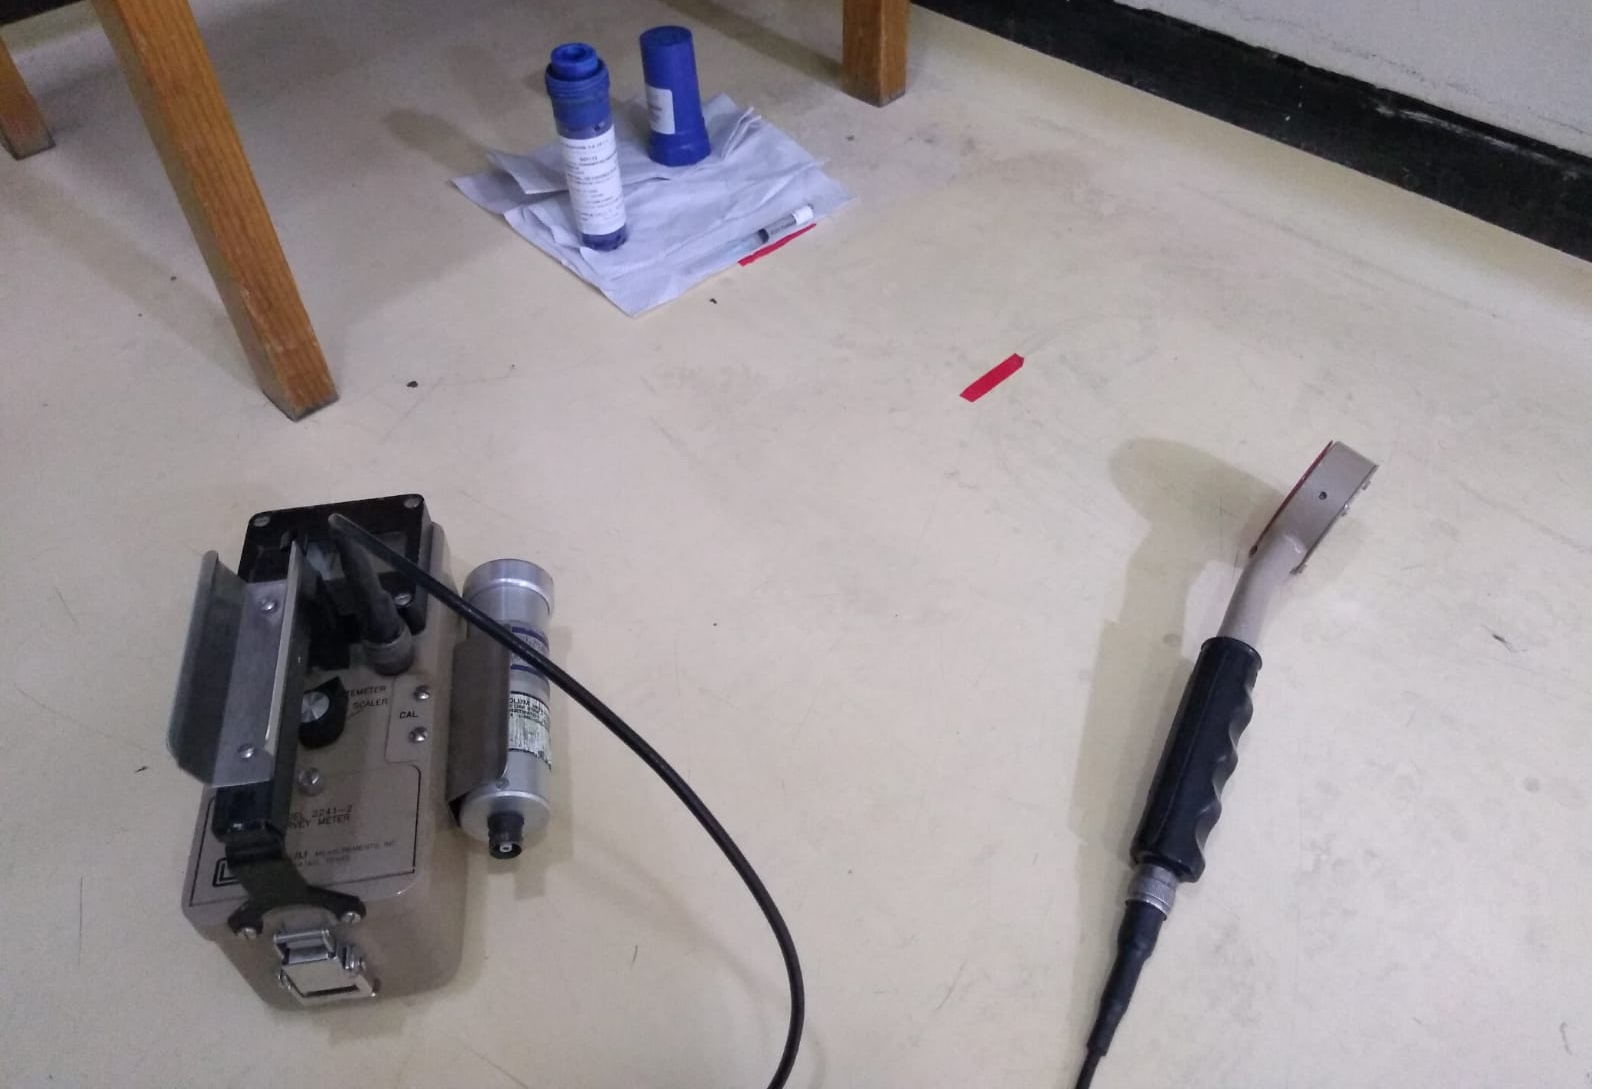
\includegraphics[width=0.45\textwidth]{./figuras/fig4.png}
    \caption{Detector Geiger-Muller en operación.}
    \label{fig:gm}
  \end{figure}



  \subsection*{Detector Geiger Muller}




Los detectores Geiger-Muller (G-M) fueron introducidos por Hans Geiger y Walter Muller en 1928, el cual en su forma más simple consiste en un tubo metálico hermético el cual contenía un gas que se ioniza liberando un electrón al interactuar con una partícula o fotón, el cual se le denomina gas de conteo \citep{detec2}. 

De manera interna contiene un ánodo que está suspendido en el centro del tubo y en la pared del mismo se encuentra el cátodo. Si el voltaje es suficientemente alto entre el ánodo y el cátodo, entonces cualquier radiación que interactúe con el gas producirá un pulso eléctrico el cual podrá ser registrado por el sistema de conteo, de esta manera este tipo de detector no es capaz de distinguir entre radiación \ec{\alpha}, \ec{\beta} o \ec{\gamma}. Los detectores Geiger-Muller de Pancake su tubo tiene forma de \textit{panqueque}, éste se muestra en la figura \ref{fig:gm}  \citep{detec1,detec2}. 
 
\subsection*{Tecnecio-99m}

El tecnecio-99m es un radionúclido empleado principalmente para fines de diagnóstico e imagenología de tejido biológico con una vida media corta de 6 horas. Su estado metaestable le permite decaer a uno estable por emisión de fotones cuyo fotopico de energía es de \ec{140.5\un{keV}} \citep{tc99m}.



\begin{figure*}[hbt]
  \centering
  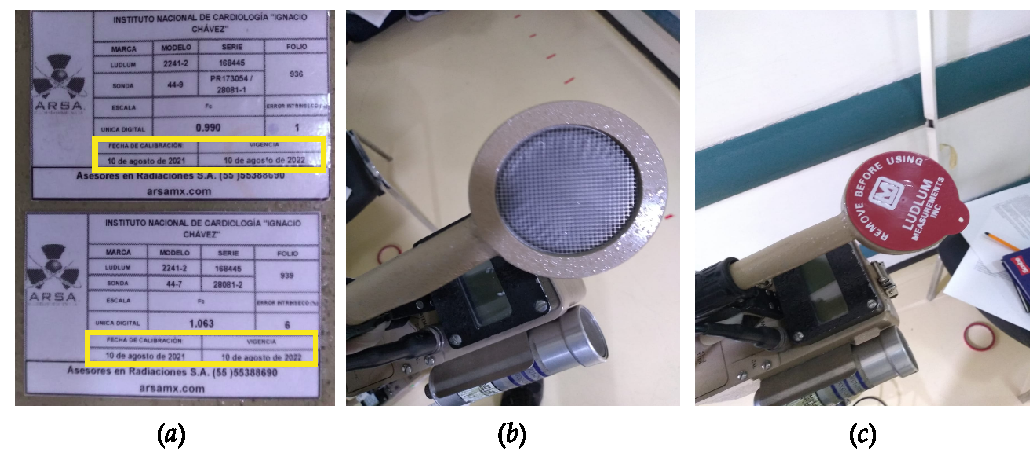
\includegraphics[width=0.95\textwidth]{./figuras/fig_meto.pdf}
  \caption{Exposición registrado en el detector.}
  \label{fig:meto}
\end{figure*}

\begin{figure*}[hbb]
  \centering
  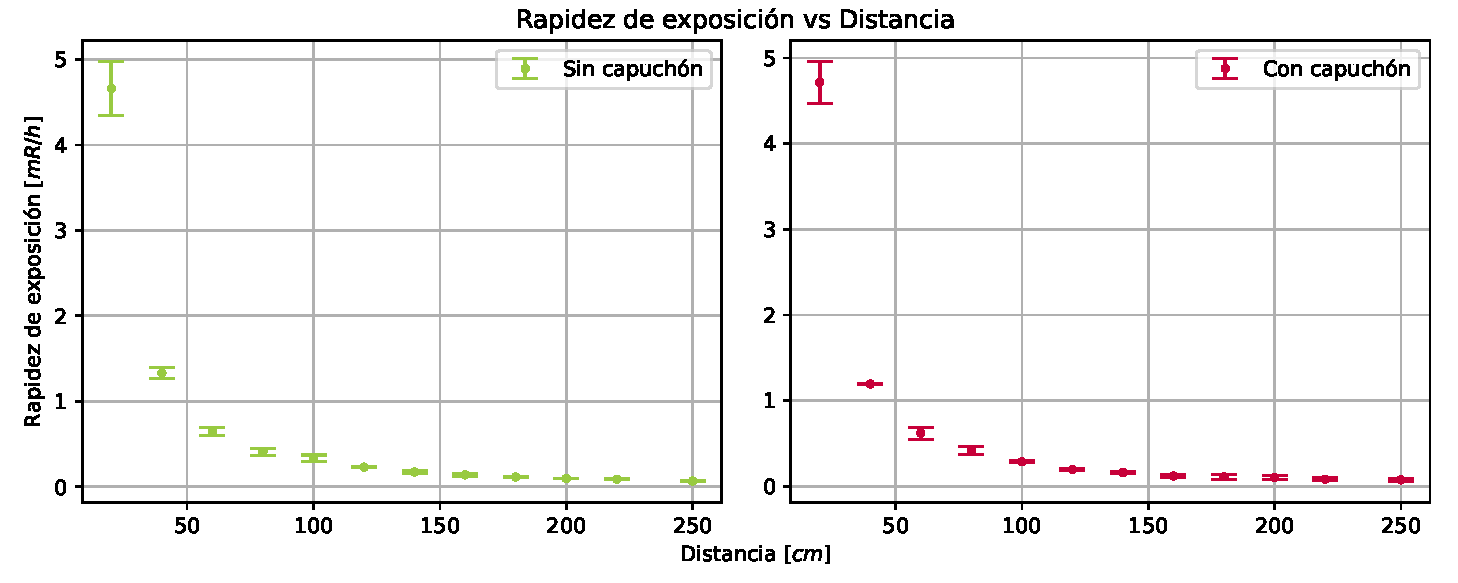
\includegraphics[width=0.95\textwidth]{./figuras/fig_sin_con.pdf}
  \caption{Rapidez de exposición \ec{\dot{X}} registrado en el detector.}
  \label{fig:pract_03_con_sin}
\end{figure*}

  \section*{Metodología}

El experimento se realizó en las instalaciones del Instituto Nacional de Cadiología ``Ignacio Chávez'' de la Ciudad de México en el departamento de Cardiología Nuclear. El manejo de la fuente sellada de tecnecio-99m requirió el uso de bata y guantes de látex.

De acuerdo la figura \hyperref[fig:meto]{\ref{fig:meto}.(a)} el detector G-M de pancake  fue calibrado el 10 de agosto de 2021 y tiene una vigencia de un año, por lo que puede ser operado. La marca del detector es LUDLUM con modelo 2241-2 y número de serie 168445, éste incluía una tapa (capuchón) el cual protege el tubo del pancake de golpes. 

Para realizar las medidas de la fuente de tecnecio-99m, se marcó el suelo con cinta adhesiva (de rojo en la figura \ref{fig:gm}) con separación de \ec{20 \un{cm}} hasta \ec{220 \un{cm}} y una adicional hasta tener una marca de \ec{250 \un{cm}}.  En la figura \hyperref[fig:meto]{\ref{fig:meto}.(b)} se muestra al detector sin capuchón, mientas que en la figura \hyperref[fig:meto]{\ref{fig:meto}.(c)} se muestra con capuchón.


%\pagebreak



  \section{Resultados  y discusiones}

Las tres series de datos tanto con y sin capuchón, los cuales fueron promediados, se muestran en la figura \ref{fig:pract_r2}. Para realizar la comparación ambas curvas se calculó el error de las medidas sin capuchón con respecto a las medidas con capuchón mediante la ecuación \ref{eq:06} los cuales se muestran en la tabla \ref{tab:1}.

\eq{eq:06}{\tx{error}_{\dot{X}}=\frac{|\dot{X}_{con}-\dot{X}_{sin}|}{\dot{X}_{con}}}
\eq{eq:07}{\tx{error}_{\dot{X}/d}=\frac{\abs{\sqrt{\frac{\dot{X}_{n+1}}{\dot{X}_n}}-\frac{d_{n}}{d_{n+1}}}}{\frac{d_{n}}{d_{n+1}}}}
De acuerdo a la ley de inversos cuadrados se puede obtener el cociente de la ecuación \ref{eq:04} con la rapidez de exposición medido experimentalmente y el vector de distancia, suponiendo \ec{A} y \ec{\Gamma} como constantes. De esta manera se puede obtener el error del cociente de la rapidez de exposición con respecto a al cociente de distancias, descrito en las ecuación \ref{eq:07}, de igual manera los datos se muestran en la tabla \ref{tab:1}.





\begin{figure*}[hbt]
    \centering
    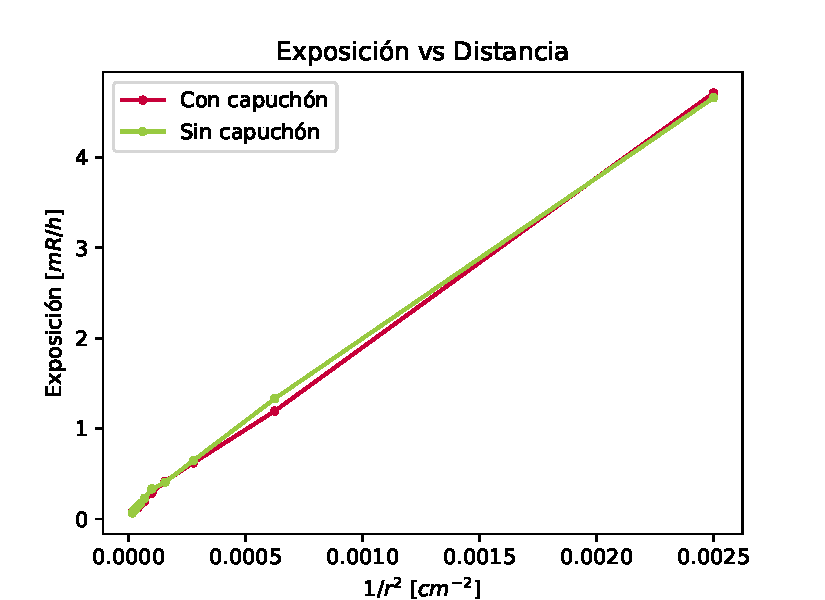
\includegraphics[width=0.99\textwidth]{./figuras/pract_03_code0_rep_r2.pdf}
    \caption{Linealización por cambio de escala del inverso cuadrado de la distancia.}
    \label{fig:pract_r2}
  \end{figure*}


  \begin{table*}[t]
    \begin{adjustbox}{width=\textwidth,center}
    \centering
    \begin{tabular}{c|c|c|c|c|c|c|c|c|c|c|c|c}
       & med1 & med2 & med3 & med4 & med5 & med6 & med7 & med8 & med9 & med10 & med11 & med12    \\\hline
       \ec{\frac{|\dot{X}_{con}-\dot{X}_{sin}|}{\dot{X}_{con}}} & 1.14\%&10.28\%&4.12\%&2.05\%&14.16\%&14.53\%&6.45\%&13.08\%&1.77\%&6.97\%&5.75\%&12.76\% \\ \hline
       & \ec{n=1} & \ec{n=2} & \ec{n=3} & \ec{n=4} & \ec{n=5} & \ec{n=6} & \ec{n=7} & \ec{n=8} & \ec{n=9} & \ec{n=10} & \ec{n=11} & -    \\
       \ec{{\sqrt{\frac{\dot{X}_{n+1}}{\dot{X}_n}}}_{con}}&0.503&0.721&0.817&0.829&0.829&0.903&0.866&0.963&0.96&0.895&0.948& -\\
       \ec{{\sqrt{\frac{\dot{X}_{n+1}}{\dot{X}_n}}}_{sin}}&0.534&0.697&0.792&0.904&0.831&0.863&0.898&0.906&0.92&0.954&0.867& -\\
       \ec{\frac{d_n}{d_{n+1}}}&0.5&0.667&0.75&0.8&0.833&0.857&0.875&0.889&0.9&0.909&0.88& -\\
      \ec{{\frac{\abs{\sqrt{\frac{\dot{X}_{n+1}}{\dot{X}_n}}-\frac{d_{n}}{d_{n+1}}}}{\frac{d_{n}}{d_{n+1}}}}_{con}} & 0.63\%&8.12\%&9.0\%&3.67\%&0.49\%&5.3\%&1.06\%&8.35\%&6.69\%&1.53\%&7.71\%& -\\ 
      \ec{{\frac{\abs{\sqrt{\frac{\dot{X}_{n+1}}{\dot{X}_n}}-\frac{d_{n}}{d_{n+1}}}}{\frac{d_{n}}{d_{n+1}}}}_{sin}} & 6.85\%&4.59\%&5.65\%&13.04\%&0.27\%&0.64\%&2.64\%&1.92\%&2.23\%&4.9\%&1.53\%& -\\

    \end{tabular}
  \end{adjustbox}
    \caption{Lista de datos y errores.}
    \label{tab:1}
  \end{table*}





  \section{Conclusiones} 

  Los registros de la tabla \ref{tab:1} muestran que las medidas con el detector con y sin capuchón son muy similares, ya que su porcentaje de error es muy bajo y esto indica que la radiación gamma es mínimamente o no atenuada por el capuchón. 
  
  Además, los ajustes lineal de los datos empleando la ley de inversos cuadrados proporcionan una R cuadrada de 0.9732 para los datos con el capuchón y 0.9557 para los datos sin éste, indicando una buena tendencia lineal. 

  Por último, puede volverse a tener la similitud entre ambos conjunto de datos en la tabla \ref{tab:1} al observar el error la raíz cuadrada del cociente de la rapidez de exposición con respecto a la distancia, de los cuales se obtienen errores muy bajos.

 \bigskip\bigskip\bigskip\bigskip
 \bigskip
 \bigskip
 \bigskip


\small{\bibliographystyle{apalike}
\bibliography{bib}}


\begin{figure}[H]
  \centering
  \qrcode[height=3cm]{https://drive.google.com/drive/folders/13PmgP-4thSk1ruKukwwLjd-M1DLD013e?usp=sharing}
  %\captionsetup{labelformat=empty}
  \caption{Código QR para acceso a los scripts de Python (solo cuentas Ciencias UNAM).}
  \label{fig:QR}
\end{figure}





\end{multicols}



%\ftikz{1.5}{figuras/fig.tikz}{}{fig:x}

\end{document}



